\documentclass{article}
\usepackage[utf8]{inputenc}
\usepackage[portuguese]{babel}
\usepackage[T1]{fontenc}
\usepackage{amsmath}
\usepackage{amsfonts}
\usepackage{amssymb}
\usepackage{amsthm}
\usepackage{framed}
\usepackage{indentfirst}
\usepackage{graphicx}
\usepackage{fancyvrb}
\usepackage{tabularx}
\usepackage{datetime}
\usepackage{algorithmic}
\usepackage[boxed]{algorithm}
\usepackage{anysize}
\usepackage{alltt}
\usepackage{sbc-template}
\usepackage{url,longtable,booktabs}

\begin{document}

\title{Implementação eficiente em \emph{software}\\ da função Lyra2 em arquiteturas modernas}

\author{Guilherme P. Gonçalves\inst{1}, Diego F. Aranha\inst{1}}

\address{Laboratório de Segurança e Criptografia (LASCA)\\
	Instituto de Computação (IC) -- Universidade Estadual de Campinas (Unicamp)\\
	Av. Albert Einsten, 1251 -- Campinas -- SP -- Brasil
	\email{guilherme.p.gonc@gmail.com,dfaranha@ic.unicamp.br}
}

\maketitle

\begin{abstract}
Password authentication has become even more challenging with the significant increase
in available computing power by means of dedicated hardware and GPUs. This work
presents an efficient software implementation of the password hashing scheme Lyra2 in modern Intel platforms,
according to version 2.5 of its specification. The resulting implementation employs
AVX2 vector instructions for a performance improvement of 30\% over the reference
implementation. In practice, it is important to know the precise performance of such primitives to inform
parameter choice and corresponding security guarantees.
\end{abstract}

\begin{resumo}
O problema de autenticação por senha tem se tornado cada vez mais desafiador, face ao crescimento
significativo de poder computacional na forma de \emph{hardware} dedicado e placas gráficas.
Este trabalho apresenta uma implementação eficiente em \emph{software} do esquema de hash de senhas Lyra2 em arquiteturas Intel modernas,
conforme a versão 2.5 de sua especificação. A implementação resultante emprega instruções vetoriais AVX2
para ganhos de desempenho em torno de 30\% sobre a implementação de referência. Na prática, é importante
determinar precisamente o desempenho de primitivas dessa natureza para informar a escolha de parâmetros
e garantias de segurança correspondentes.
\end{resumo}

\section{Introdução}

A forma mais comum de autenticação de usuários em sistemas
computacionais atualmente é o uso de senhas. Nesse paradigma, o usuário
é responsável por escolher uma senha ao se registrar, que deve
permanecer secreta, e o sistema verifica, a cada acesso, se o usuário
conhece a senha correta. Isso implica, é claro, o armazenamento da senha
de alguma forma no sistema.

Como medida de segurança, recomenda-se não armazenar a senha conforme
fornecida pelo usuário, mas sim um \emph{hash} produzido por um esquema
de \emph{hash} de senhas. O \emph{hash} produz uma sequência pseudoaleatória
de \emph{bits} tal que, dado o valor de \emph{hash} $h$ de uma senha
$s$, deve ser computacionalmente difícil descobrir qualquer senha
(incluindo $s$) cujo \emph{hash} também seja $h$ -- uma propriedade
conhecida como resistência ao cálculo de pré-imagem.
Assim, em um procedimento de autenticação moderno, o sistema calcula o
\emph{hash} da senha provida pelo usuário e o compara com o \emph{hash}
que havia sido armazenado para aquele usuário ao registrá-lo. Caso os
\emph{hashes} sejam iguais, o acesso é autorizado.

Muitas técnicas foram introduzidas para dificultar
ataques de busca exaustiva -- aqueles em que um atacante faz tentativas
sucessivas de adivinhar uma senha -- sem onerar usuários exigindo que
criem e memorizem senhas longas e suficientemente entrópicas.
No campo dos esquemas de \emph{hash} de senhas, isso significa a inclusão
de parâmetros de tempo e espaço de memória mínimos a serem utilizados
pela operação de \emph{hash}. O parâmetro de tempo impõe um limite à
velocidade com que um atacante pode fazer tentativas sequenciais,
enquanto o de espaço visa a proteger contra ataques que empregam \emph{hardware}
dedicado ou GPUs, caracterizados pelo paralelismo e escassez de memória.

Neste trabalho, foi produzida uma implementação do
esquema de \emph{hash} de senhas Lyra2, proposta por pesquisadores
brasileiros e finalista do \emph{Password Hashing Competition}\footnote{\url{https://password-hashing.net/}}, aproveitando
conjuntos de instruções presentes em arquiteturas modernas. Acredita-se
que o Lyra2 possua as propriedades de segurança exigidas de um esquema
de \emph{hash} de senhas, e sua especificação inclui parâmetros de espaço e tempo
independentes a serem respeitados por uma implementação correta.
A implementação resultante\footnote{Disponível em \url{https://github.com/guilherme-pg/lyra2}}
é compatível com a de referência e competitiva em termos de desempenho. Houve colaboração
ainda com o desenvolvimento da especificação do Lyra2 \cite{lyra2-spec},
na medida em que este trabalho trouxe à tona diversas
inconsistências no documento de especificação e na implementação de referência.

A implementação proposta possui duas variantes: uma utilizando as instruções
vetoriais do conjunto SSE2, e outra utilizando as do conjunto AVX2. Como o
código de referência possui versões genérica (sem instruções vetoriais) e SSE2,
cabe clarificar que, para o restante deste documento, quaisquer menções à
implementação proposta ou à de referência se aplicam às respectivas versões
SSE2 (a não ser, é claro, que a versão AVX2 deste trabalho esteja sendo
discutida).

\section{Notação}

Para o restante deste documento, os símbolos da primeira coluna da
Tabela~\ref{tb:notation} a seguir serão usados com o significado dado pela segunda coluna.

\begin{longtable}[c]{@{}cc@{}}
\toprule
Símbolo & Significado\tabularnewline
\midrule
\endhead
$\oplus$ & XOR bit-a-bit\tabularnewline
$\lfloor \cdot \rfloor l$ & Truncagem para $l$ \emph{bits}\tabularnewline
$\ggg n$ & Rotação $n$ \emph{bits} à direita\tabularnewline
$\boxplus$ & Adição sem carry entre palavras\tabularnewline
$||$ & Concatenação\tabularnewline
$len(n)$ & Tamanho em bytes de $n$\tabularnewline
$LSW(n)$ & Palavra menos significativa de $n$\tabularnewline
$rotRt(n)$ & Rotação $Rt$ \emph{bits} à direita de $n$\tabularnewline
$rotRt^{m}(n)$ & Rotação $m \cdot Rt$ \emph{bits} à direita de
$n$\tabularnewline
\bottomrule
\caption{\label{tb:notation} Notação utilizada neste trabalho.}
\end{longtable}
\vspace{-1cm}

\section{O esquema de hash Lyra2}

O Lyra2 se baseia na construção de esponja, uma forma geral para a
geração de funções de \emph{hash} seguras com entradas e saídas de
tamanhos arbitrários a partir de uma função de compressão e um esquema
de \emph{padding}. De fato, o cálculo do Lyra2 para uma determinada entrada pode ser
descrito em alto nível como a aplicação iterada de operações de esponja,
a serem descritas a seguir, a dados mantidos em uma matriz de estado do
algoritmo. Consequentemente, conjectura-se que as propriedades de
segurança do Lyra2 decorrem tanto da segurança da esponja subjacente,
quanto da escolha criteriosa de operações de esponja empregadas, que
dificulta a paralelização do algoritmo.

\subsection{A construção de esponja}

A definição canônica de uma esponja \cite{sponge} descreve sua operação
em termos de duas etapas -- \emph{absorbing} e \emph{squeezing} --,
sendo que na primeira a esponja incorpora a entrada a seu estado
interno, e na segunda produz uma saída do tamanho desejado baseada nesse
estado. Assim, ao final de uma etapa de \emph{squeezing}, a esponja terá
produzido um \emph{hash} pseudoaleatório de sua entrada, e pode ser
restaurada a seu estado original para uma aplicação posterior.

A Figura \ref{img-sponge} ilustra a construção de esponja. Nela, a
entrada $M$ é dividida em blocos após o \emph{padding} e absorvida
para gerar a saída $Z$. $f$ é uma função de compressão. A linha
tracejada separa as etapas de \emph{absorbing} (esquerda) e
\emph{squeezing} (direita), e o estado interno da esponja é dividido em
duas partes com tamanhos $r$ (taxa) e $c$ (capacidade)
\emph{bits}.

\begin{figure}[htbp]
\centering
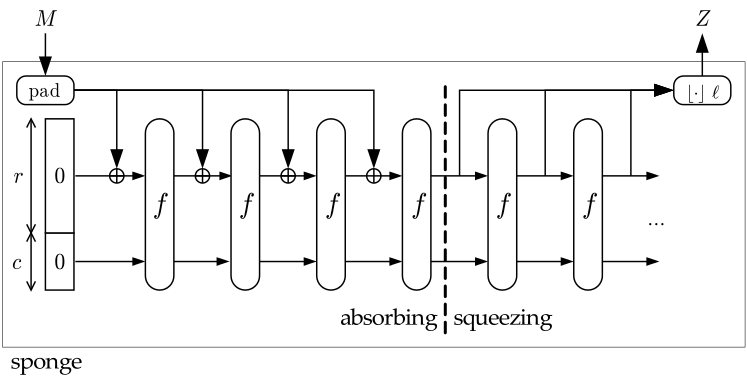
\includegraphics{./img/sponge.png}
\caption{A construção de esponja, adaptado de~\cite{sponge}.\label{img-sponge}}
\end{figure}

Pode-se definir, ainda, uma construção similar à da esponja, denominada
\emph{duplex}, em que se mantém o estado interno entre aplicações. Nela,
as operações de \emph{absorb} e \emph{squeeze} são substituídas por uma
operação de \emph{duplexing}, na qual um bloco de entrada é absorvido e
um bloco de saída é imediatamente produzido. A Figura \ref{img-duplex}
ilustra a construção de \emph{duplex}.

\begin{figure}[htbp]
\centering
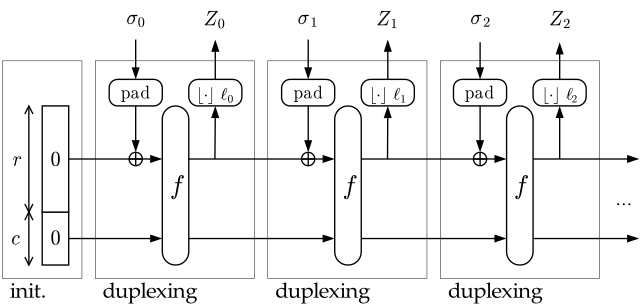
\includegraphics{./img/duplex.png}
\caption{A construção de duplex, adaptado de~\cite{sponge}.\label{img-duplex}}
\end{figure}

O Lyra2 utiliza uma versão modificada da construção de \emph{duplex}, em
que as operações de \emph{absorb} e \emph{squeeze} também são
suportadas, e podem ser efetuadas independentemente.

\subsection{A função de compressão}\label{sec-compression-fn}

Conforme visto anteriormente, a construção de esponja depende de uma
função $f$, denominada função de compressão. Para a esponja usada no
Lyra2, a função de compressão é uma versão levemente adaptada da função
$G$ que integra a função de \emph{hash} BLAKE2b \cite{blake2b} . A função
$G(a, b, c, d)$ utilizada é dada por:
\begin{align*}
\begin{split}
& a \leftarrow a + b \\
& d \leftarrow \left(d \oplus a \right) \ggg 32 \\
& c \leftarrow c + d \\
& b \leftarrow \left(b \oplus c \right) \ggg 24 \\
& a \leftarrow a + b \\
& d \leftarrow \left(d \oplus a \right) \ggg 16 \\
& c \leftarrow c + d \\
& b \leftarrow \left(b \oplus c \right) \ggg 63
\end{split}
\end{align*}

No contexto do algoritmo BLAKE2b, essa função é aplicada repetidamente a
uma matriz de estado $4 \times 4$ de inteiros de 64 \emph{bits},
primeiramente aos elementos de cada uma das colunas, depois aos de cada
uma das diagonais. Essas oito aplicações constituem uma \emph{rodada}, e
o algoritmo prevê transformações de seu estado em conjuntos de 12
rodadas por vez.

No Lyra2, o estado da esponja contém $128$ bytes e é visto como uma
matriz de estado linearizada, e as rodadas são definidas de forma
análoga. No entanto, a fim de melhorar o desempenho do algoritmo, a
maior parte das compressões efetuadas pela esponja não utiliza
$\rho_{max} = 12$ rodadas, mas sim $\rho < \rho_{max}$ (na prática,
utiliza-se $\rho = 1$). Tais operações com apenas $\rho$ rodadas são
denominadas operações \emph{reduzidas} da esponja.

\subsection{O algoritmo Lyra2 }\label{sec-lyra2-alg}

A Figura \ref{lyra2-alg} contém o pseudocódigo do algoritmo Lyra2
implementado para este trabalho. Basicamente, o algoritmo consiste de três etapas: \emph{bootstrapping},
\emph{setup} e \emph{wandering}. Todas elas trabalham sobre uma matriz
de estado de $R \times C$ blocos de $b$ \emph{bits}, onde $R$ e $C$
são, portanto, parâmetros de espaço.

\begin{figure}[htbp]
\centering
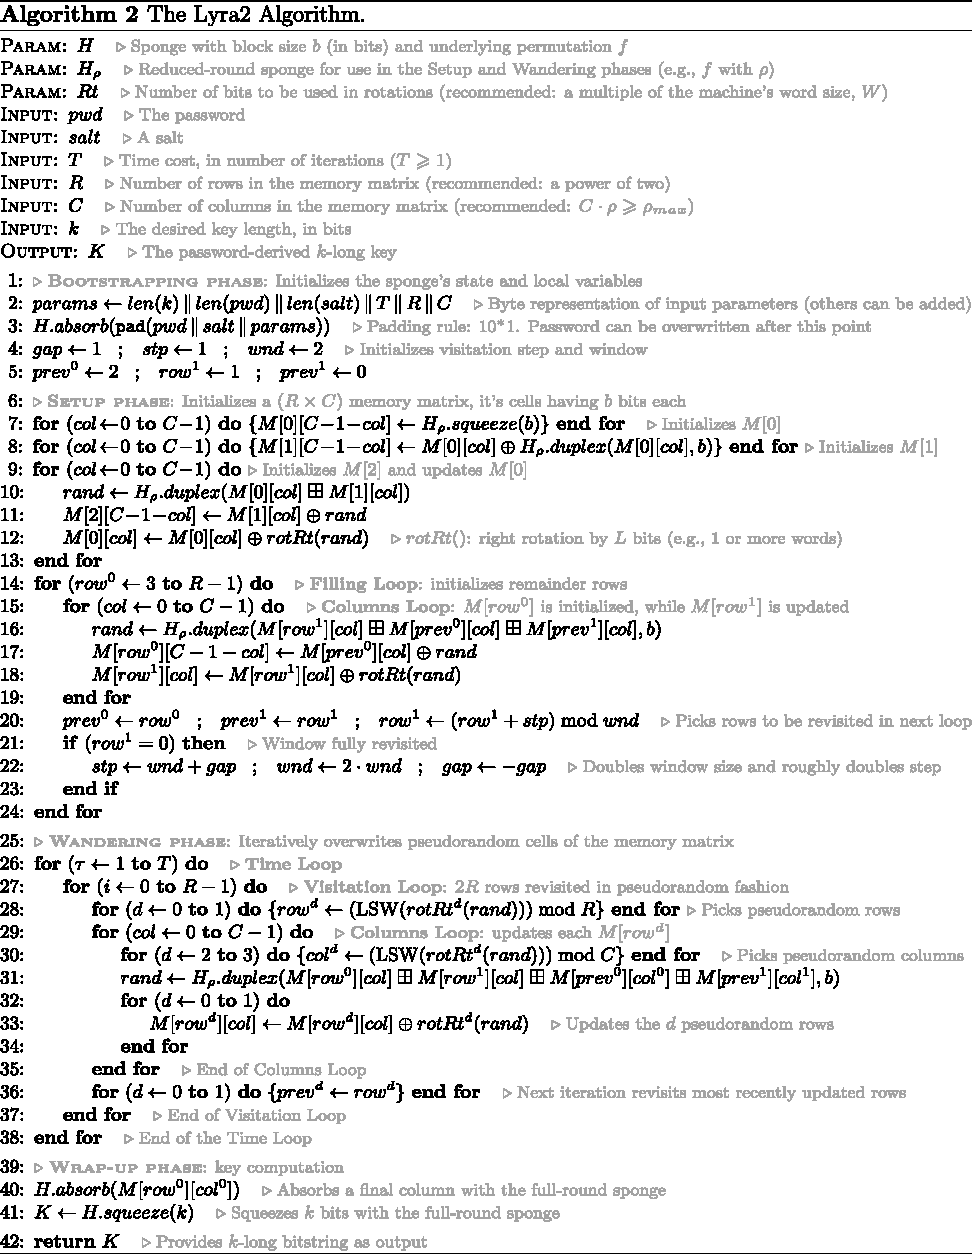
\includegraphics[width=\linewidth]{./img/spec.pdf}
\caption{O algoritmo Lyra2 implementado neste trabalho\label{lyra2-alg}, conforme versão 2.5 da especificação~\cite{lyra2-spec}.}
\end{figure}

O tamanho dos blocos é definido de forma que possam ser absorvidos sem
\emph{padding} pela esponja utilizada. Embora um bloco de $b = r$ \emph{bits}
pareça natural tendo em vista as Figuras \ref{img-sponge} e
\ref{img-duplex}, a especificação sugere aumentar $r$ após a primeira
absorção (linha 3 da Figura \ref{lyra2-alg}). Na prática, tanto no
código desenvolvido quanto no de referência utilizam um $r$ inicial de $512$ \emph{bits},
e utilizam posteriormente um novo $r = b = 768$ \emph{bits}.

A fase de \emph{bootstrapping} inicializa a esponja com o vetor de
inicialização da função de compressão, e então absorve os parâmetros de
entrada. A fase de \emph{setup} inicializa a matriz de estado, e a fase
de \emph{wandering} aplica operações reduzidas de esponja a células
pseudoaleatórias dessa matriz. Nessa fase, o parâmetro $T$ controla o
número de iterações a serem feitas, e, portanto, o tempo utilizado.
O tempo total de execução do algoritmo é dado por
$(T + 1) \cdot R \cdot C \cdot \frac{\rho}{\rho_{max}}$ vezes o tempo
de execução da função de compressão da esponja, de forma que, ainda que
o tempo de execução seja limitado inferiormente pelos parâmetros de
memória $R$ e $C$, ainda é possível aumentá-lo mantendo o consumo de
memória constante, através do parâmetro $T$.

\section{Descrição da implementação}

A implementação proposta foi desenvolvida, tal como a de referência, utilizando
a linguagem C, mas com base em decisões de projeto levemente diferentes. Além
de prezar pelo desempenho, o trabalho foi desenvolvido com particular cuidado
pela legibilidade, facilitando eventuais auditorias do código, e portabilidade,
evitando-se utilizar extensões específicas de determinados compiladores e
aderindo-se de forma bastante estrita ao padrão C99.

Uma diferença particularmente perceptível entre as implementações é que,
enquanto a de referência utiliza largamente \emph{intrinsics} para obter
controle fino sobre as instruções geradas, a implementação mantém os
operadores de alto nível da linguagem C e delega ao compilador a tarefa
de emitir as instruções vetoriais para a maior parte do código, à
exceção da função de compressão. Além do benefício em legibilidade, essa
decisão tornou prático emitir versões utilizando diferentes conjuntos de
instruções usando o mesmo código, e, conforme a Seção
\ref{sec-experimental}, não trouxe perda de desempenho significativa.

O código utilizado para a função de compressão é o da implementação de
referência da BLAKE2b \footnote{Disponível em
  \url{https://github.com/BLAKE2/BLAKE2}}, com pequenas adaptações para
remover as constantes utilizadas durante aplicações da função $G$. No
entanto, como essa implementação da BLAKE2b não possui versão AVX2, foi
necessário adaptá-la conforme descrito na Subseção \ref{sec-compression-fn-avx2}
para que utilizasse esse conjunto de instruções.

O algoritmo Lyra2 apresentado na Subseção \ref{sec-lyra2-alg} não
especifica o parâmetro $Rt$, que determina o tamanho em \emph{bits} das
rotações de blocos; a implementação de referência, em sua versão SSE2,
utiliza $Rt = 128$ \emph{bits}, dado que este é o tamanho de um vetor SSE2.
Da mesma forma, o trabalho usa $Rt = 128$ quando compilado com
SSE2, e $Rt = 256$ em sua versão AVX2.

\subsection{A função de compressão em AVX2 }\label{sec-compression-fn-avx2}

Esta seção detalha as mudanças feitas na implementação de referência da
função de compressão do Lyra2 para aproveitar as instruções vetoriais do
conjunto AVX2.

Conforme exposto na Subseção \ref{sec-compression-fn}, a função de
compressão do Lyra2 consiste de $\rho$ rodadas da função $G$ sobre uma
matriz de estado $4 \times 4$ de $64$ \emph{bits}. Assim, para uma matriz
da forma:
\begin{align*}
\left(
\begin{matrix}
v_{0} & v_{1} & v_{2} & v_{3} \\
v_{4} & v_{5} & v_{6} & v_{7} \\
v_{8} & v_{9} & v_{10} & v_{11} \\
v_{12} & v_{13} & v_{14} & v_{15}
\end{matrix}
\right)
\end{align*}
uma rodada corresponde a:
\begin{align*}
\begin{matrix}
G(v_{0}, v_{4}, v_{8}, v_{12}) & G(v_{1}, v_{5}, v_{9}, v_{13}) & G(v_{2}, v_{6}, v_{10}, v_{14}) & G(v_{3}, v_{7}, v_{11}, v_{15}) \\
G(v_{0}, v_{5}, v_{10}, v_{15}) & G(v_{1}, v_{6}, v_{11}, v_{12}) & G(v_{2}, v_{7}, v_{8}, v_{13}) & G(v_{3}, v_{4}, v_{9}, v_{14})
\end{matrix}
\end{align*}
onde as aplicações em cada linha podem ocorrer em paralelo. No caso do
Lyra2, o estado da esponja possui $16 \times 64 = 1024$ \emph{bits} e é
interpretado como uma matriz de estado linearizada em ordem de linhas
para os propósitos da função de compressão.

Na implementação vetorizada de referência da BLAKE2b, cada registrador
vetorial corresponde a mais de um inteiro de $64$ \emph{bits} da matriz de
estado -- por exemplo, em uma implementação SSE2, $v_{0}$ e $v_{1}$
compartilham um registrador de $128$ \emph{bits}. Uma rodada consiste então
em executar a função $G$ sobre as linhas da matriz em paralelo, rotacionar
a $i$-ésima linha da matriz de estado por $i$ posições à esquerda, de forma
que as antigas diagonais se tornem as colunas, aplicar a função $G$ sobre
as (novas) colunas, e desfazer as rotações~\cite{blake2b}. O
procedimento de rotação das linhas é chamado de \emph{diagonalização}.

Dessa forma, uma versão AVX2 da função de compressão pode utilizar as
mesmas técnicas que uma versão SSE2, adaptadas para o fato de que os
registradores de $256$ \emph{bits} comportam uma linha inteira da matriz de
estado por vez. Especificamente, o código AVX2 produzido para este
trabalho utiliza as novas instruções \texttt{vpaddq} para as adições de
$64$ \emph{bits}, \texttt{vpxor} para as operações de XOR, \texttt{vpshufd} e
\texttt{vpshufd} para as rotações, e \texttt{vpermq} para as rotações de
linhas da matriz.

Em termos de código, a implementação AVX2 possui a mesma estrutura
geral que a de referência, apesar do uso de \emph{intrinsics}
diferentes. A função $G$ é dividida nas partes G1 e G2: G1 contém as
instruções até a rotação de 24 \emph{bits} à direita, e G2 contém o restante da
função. G1 e G2 são implementadas conforme a listagem a seguir:

\begin{small}
\begin{verbatim}
#define G1(row1,row2,row3,row4)		\
  row1 = _mm256_add_epi64(row1, row2);	\
  row4 = _mm256_xor_si256(row4, row1);	\
  row4 = _mm256_roti_epi64(row4, -32);	\
  row3 = _mm256_add_epi64(row3, row4);	\
  row2 = _mm256_xor_si256(row2, row3);	\
  row2 = _mm256_roti_epi64(row2, -24);	\

#define G2(row1,row2,row3,row4)		\
  row1 = _mm256_add_epi64(row1, row2);	\
  row4 = _mm256_xor_si256(row4, row1);	\
  row4 = _mm256_roti_epi64(row4, -16);	\
  row3 = _mm256_add_epi64(row3, row4);	\
  row2 = _mm256_xor_si256(row2, row3);	\
  row2 = _mm256_roti_epi64(row2, -63);	\
\end{verbatim}
\end{small}

Cabe notar que, na listagem acima, \texttt{\_mm256\_roti\_epi64},
responsável pelas rotações, é a única primitiva que não é um
\emph{intrinsic}. Essa macro é definida como:

\begin{small}
\begin{verbatim}
#define r16_256 _mm256_setr_epi8(                              \
    2, 3, 4, 5, 6, 7, 0, 1, 10, 11, 12, 13, 14, 15, 8, 9, 18,  \
    19, 20, 21, 22, 23, 16, 17, 26, 27, 28, 29, 30, 31, 24, 25)
#define r24_256 _mm256_setr_epi8(                              \
    3, 4, 5, 6, 7, 0, 1, 2, 11,12, 13, 14, 15, 8, 9, 10, 19,   \
    20, 21, 22, 23, 16, 17, 18, 27, 28, 29, 30, 31, 24, 25, 26)
\end{verbatim}
\end{small}
\newpage
\begin{small}
\begin{verbatim}
#define _mm256_roti_epi64(x, c)                                    \
    (-(c) == 32) ? _mm256_shuffle_epi32((x), _MM_SHUFFLE(2,3,0,1)) \
    : (-(c) == 24) ? _mm256_shuffle_epi8((x), r24_256)             \
    : (-(c) == 16) ? _mm256_shuffle_epi8((x), r16_256)             \
    : (-(c) == 63) ? _mm256_xor_si256(_mm256_srli_epi64((x), -(c)),\
                                      _mm256_add_epi64((x), (x)))  \
    : _mm256_xor_si256(_mm256_srli_epi64((x), -(c)),               \
                       _mm256_slli_epi64((x), 64-(-(c))))}
\end{verbatim}
\end{small}

A diagonalização e sua inversa são implementadas a partir do \emph{intrinsic}
de permutação de palavras \texttt{\_mm256\_permute4x64\_epi64}, definido como abaixo:

\begin{small}
\begin{verbatim}
#define DIAGONALIZE(row1, row2, row3, row4)                   \
  row2 = _mm256_permute4x64_epi64(row2, _MM_SHUFFLE(0,3,2,1));\
  row3 = _mm256_permute4x64_epi64(row3, _MM_SHUFFLE(1,0,3,2));\
  row4 = _mm256_permute4x64_epi64(row4, _MM_SHUFFLE(2,1,0,3));}

#define UNDIAGONALIZE(row1, row2, row3, row4)                 \
  row2 = _mm256_permute4x64_epi64(row2, _MM_SHUFFLE(2,1,0,3));\
  row3 = _mm256_permute4x64_epi64(row3, _MM_SHUFFLE(1,0,3,2));\
  row4 = _mm256_permute4x64_epi64(row4, _MM_SHUFFLE(0,3,2,1));}
\end{verbatim}
\end{small}

E, assim, uma rodada é definida como:

\begin{small}
\begin{verbatim}
#define BLAKE2B_ROUND(v)                \
  G1(v[0], v[1], v[2], v[3]);           \
  G2(v[0], v[1], v[2], v[3]);           \
  DIAGONALIZE(v[0], v[1], v[2], v[3]);  \
  G1(v[0], v[1], v[2], v[3]);           \
  G2(v[0], v[1], v[2], v[3]);           \
  UNDIAGONALIZE(v[0], v[1], v[2], v[3]);}
\end{verbatim}
\end{small}
onde o parâmetro \texttt{v} é uma matriz de estado linearizada, de forma
que \texttt{v[i]} é um \texttt{\_\_m256i} contendo a $i$-ésima linha.

Além dessas adaptações na função de compressão, as únicas mudanças
não-triviais feitas no restante do código da implementação para
habilitar nela o uso de AVX2 dizem respeito aos requerimentos de
alinhamento de memória nos operandos das novas instruções.

\section{Resultados experimentais }
\label{sec-experimental}

Esta seção apresenta os resultados de uma comparação de desempenho entre
diferentes implementações do Lyra2. Os testes foram conduzidos em
dois ambientes diferentes: um Macbook Pro Retina modelo Mid-2012 rodando
o sistema operacional OSX na versão 10.10.4, com um processador Intel
Core i7-3720QM (família Ivy Bridge) e 16 GiB de memória, e uma máquina
com processador Intel Core i7-4770 (família Haswell) e 8GiB de memória
rodando a distribuição Linux Fedora 18. O recurso TurboBoost, que
aumenta dinamicamente a frequência do processador, foi desativado em
ambas as máquinas.

A metodologia utilizada consistiu em executar cada implementação
$1000$ vezes com as mesmas entradas e extraindo-se uma senha de $64$
bytes, para três conjuntos de parâmetros $R$ e $T$ do algoritmo
Lyra2. O parâmetro $C$ foi deixado fixo em $256$, o valor sugerido
pela implementação de referência. A mediana dos tempos levados nessas
$1000$ execuções foi tomada como métrica final de desempenho, para
cada conjunto de parâmetros. Os processos foram executados usando
prioridade normal, o padrão em ambos os sistemas.

Na implementação de referência, as otimizações em tempo de ligação (\emph{link
time optimizations}) foram desativadas por causar erros de ligação no ambiente
Linux com LLVM, após constatar-se que não traziam diferença significativa de
desempenho nos testes realizados com GCC.

Para cada um dos códigos, foram testados os binários gerados pelos
compiladores LLVM e GCC, nas respectivas versões 3.4.2 e 4.9.0. No
entanto, devido ao limitado suporte ao GCC no sistema OSX, apenas
medições com LLVM foram feitas nessa plataforma. Essas medições visam a
avaliar o impacto de delegar a maior parte das escolhas de instruções
para o compilador no código, indo de encontro à abordagem da
implementação de referência, que se baseia fortemente no uso explícito
de \emph{intrinsics}.

A Figura \ref{results-linux} ilustra os resultados experimentais obtidos
no ambiente Linux. Nela, os nomes \emph{ref-gcc} e \emph{ref-clang}
correspondem à implementação de referência compilada, respectivamente,
com GCC e LLVM. Os nomes \emph{gcc} e \emph{clang} são análogos, mas
referem-se à implementação proposta neste trabalho. Finalmente,
\emph{avx2-clang} e \emph{avx2-gcc} correspondem à variante que utiliza
as instruções AVX2, descrita na Subseção \ref{sec-compression-fn-avx2},
novamente usando os dois compiladores analisados. Os tempos de execução
foram normalizados pelo da medição \emph{ref-gcc}, para cada conjunto de
parâmetros.

\begin{figure}[htbp]
\centering
\includegraphics[width=\linewidth]{./img/linux.png}
\caption{Tempos de execução normalizados para as três configurações de parâmetros em Linux\label{results-linux}.}
\end{figure}

As versões AVX2, conforme esperado, tiveram desempenho melhor do que as
demais. Nelas, o compilador utilizado não trouxe diferença significativa
(\emph{avx2-clang} foi apenas cerca de $3\%$ mais rápida do que
\emph{avx2-gcc} em todos os testes), e ambas foram cerca de $30\%$
mais rápidas do que \emph{ref-gcc} em todos os testes. Os desvios padrão
para as medições destas versões foram baixos em todos os testes: cerca de $6$,
$9$ e $18 \mu s$, respectivamente, para os testes representados na Figura
\ref{results-linux}.

A escolha do compilador influenciou sensivelmente a implementação de
referência. Para todos os conjuntos de parâmetros, \emph{ref-clang} foi cerca
de $9\%$ mais lenta do que \emph{ref-gcc}. Para a implementação deste trabalho,
no entanto, observou-se influência contrária dos compiladores, e de muito menor
magnitude: \emph{gcc} foi apenas cerca de $1.5\%$ mais lenta do que \emph{clang}
em todos os testes.

Entre as versões SSE2, \emph{clang} foi a mais rápida para todos os conjuntos
de parâmetros, com desempenho cerca de $17\%$ melhor do que \emph{ref-gcc}. A
maior diferença observada ocorreu com $R = T = 16$, em que \emph{clang} foi
$17.76\%$ mais rápida do que \emph{ref-gcc} ($1445 \mu s$ contra $1757 \mu s$).
Os desvios padrão para essas versões também se mantiveram baixos em todas as
configurações: em torno de $6$, $11$ e $20 \mu s$, respectivamente.

A Figura \ref{results-osx} mostra os resultados dos mesmos testes
executados na máquina rodando OSX. Como nela não há suporte ao conjunto
de instruções AVX2, não foi possível avaliar \emph{avx2-clang} nessa
plataforma. Aqui registrou-se significativa diferença de desempenho entre os
binários, com \emph{clang} sendo cerca de $25\%$ mais rápida do que a
implementação de referência em todos os testes.

\begin{figure}[htbp]
\centering
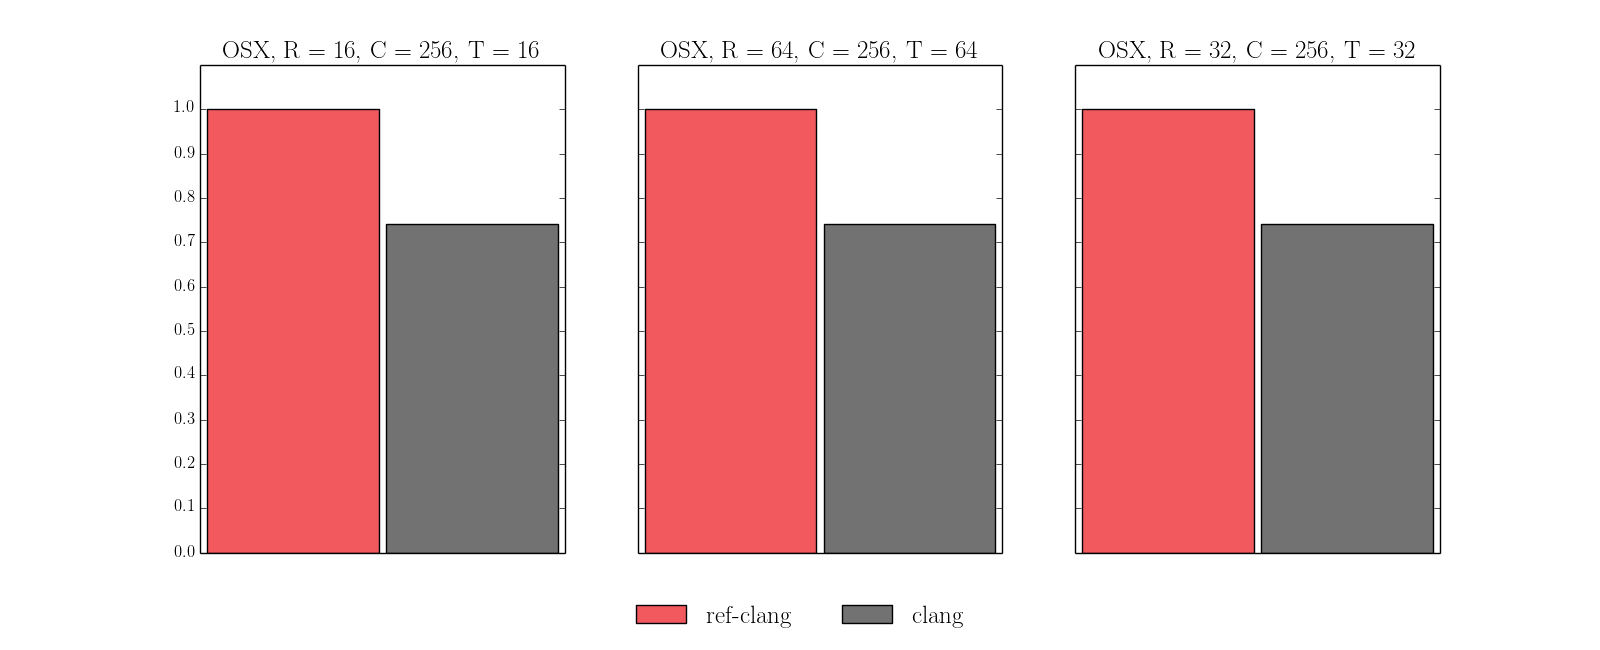
\includegraphics[width=\linewidth]{./img/osx.png}
\caption{Tempos de execução normalizados para as três configurações de
parâmetros em OSX\label{results-osx}.}
\end{figure}

Cabe notar, no entanto, que as medições no ambiente OSX apresentaram desvios
padrão bem maiores do que em Linux para ambas as implementações. No teste de
maior diferença relativa entre as implementações, $R = T = 16$, \emph{clang} foi
$26.76\%$ mais rápida do que \emph{ref-clang} ($1888 \mu s$ contra $2578 \mu
s$), com desvios padrão de $21.90 \mu s$ e $35.34 \mu s$, respectivamente. Para
o terceiro conjunto de parâmetros, $R = T = 64$, \emph{clang} teve alto desvio
padrão ($177.39 \mu s$, contra $121.31 \mu s$ de \emph{ref-clang}), mas
desempenho ainda $25.31\%$ melhor.

Dado que a implementação proposta foi desenvolvida no ambiente com OSX e
LLVM, e a de referência foi produzida em ambiente Linux com GCC,
pode-se dizer que as diferenças de desempenho entre compiladores
refletem a maior exposição de cada implementação à plataforma em que foi
escrita.

\section{Conclusão}

Este trabalho produziu uma implementação de um novo esquema de
\emph{hash} de senhas tomando proveito de arquiteturas e compiladores
modernos. A implementação é compatível e competitiva com a de
referência, tendo-se obtido significativa melhora de desempenho com o
uso conjunto de instruções AVX2, e seu desenvolvimento contribuiu com a
evolução da especificação.
É importante determinar precisamente o desempenho de primitivas dessa natureza para tanto informar a escolha de parâmetros
quanto estimar as garantias de segurança correspondentes.

\bibliographystyle{sbc}
\bibliography{lyra2}

\end{document}
